\documentclass[12pt, a4paper]{article}

\usepackage[utf8]{inputenc}
\usepackage[greek, english]{babel}
\usepackage{alphabeta}
\usepackage{libertine}
\usepackage{graphicx}
\usepackage{biblatex}[sorting=nty] % sort alphabetically
\usepackage[table]{xcolor}
\usepackage{mathptmx} % Times New Roman
\usepackage{makecell}
\usepackage{setspace}
\usepackage{geometry}

\pagenumbering{arabic}
\onehalfspacing % Set line spacing to 1.5
\graphicspath{ {./output/} }
\addbibresource{refs.bib}

\def\code#1{\texttt{#1}}

\title{\Huge Probability and statistics for data analysis\\ \LARGE 2nd Assignment }


\begin{document}
	
	\begin{titlepage}
		\maketitle
		\begin{center}
			
			\LARGE Professors: I. Vrontos
			
			\large Athens University of Economics and Business
			
			\large MSc in Data Science
			
		\end{center}
		
	\end{titlepage}
	
	\tableofcontents
	\newpage
	
	\section{ANOVA Testing}
	
	\subsection{One-way ANOVA Tests}
	
	The relationship between $W$ and $Y, X1, X2, X3, X4$ can be found in Figure \ref{fig::boxplots_1}. Specifically:
	
	\begin{itemize}
		\item There are significant differences between X1 and W  on a $90\%$ confidence level $p = 0.0915$. The normality assumptions hold on a $95\%$ confidence level (S-W $p=0.268$, K-S $p=0.1506$) and so does the homogeneity assumption (Lev $p=0.3367$).
		
		\item There are no statistically significant differences between X2 and W  on a $90\%$ confidence level $p = 0.128$. The normality assumptions hold on a $95\%$ confidence level (S-W $p=0.8049$, K-S $p=0.2343$) and so does the homogeneity assumption (Lev $p=0.3412$).
		
		\item There are no statistically significant differences between X3 and W  on a $90\%$ confidence level $p = 0.876$. The normality assumptions hold on a $95\%$ confidence level (S-W $p=0.2555$, K-S $p=0.1112$). We reject the homogeneity assumption on a $90\%$ confidence level (Lev $p=0.0007$) and as such our results may not be accurate.
		
		\item There are statistically significant differences between X2 and W on a $95\%$ confidence level $p = 0.0168$. The normality assumptions hold on a $95\%$ confidence level (S-W $p=0.4243$, K-S $p=0.4261$) and so does the homogeneity assumption (Lev $p=0.4261$).
		
	\end{itemize}
	 
	
	\begin{figure}
		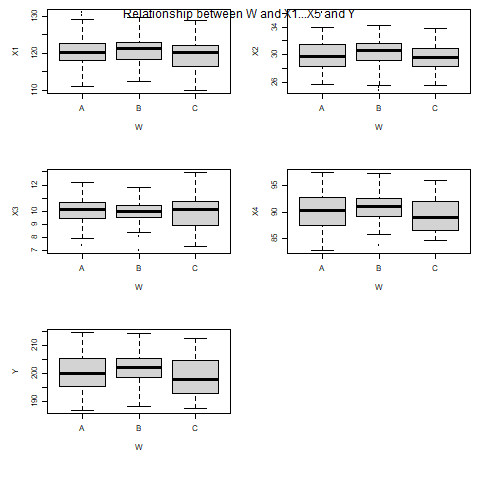
\includegraphics[width=8cm]{boxplots_1.png}
		\centering
		\caption{Boxplots of W in relation to the other variables.}
		\label{fig::boxplots_1}
	\end{figure}
	
	
	\subsection{Graphical Representation of $X_i$ effect on Y depending on W}
	
	Figure \ref{fig::scatterplot_1} shows the relation of Y with the other variables $X_i, i=1,2,3,4$ depending on W.
	
	\begin{figure}
		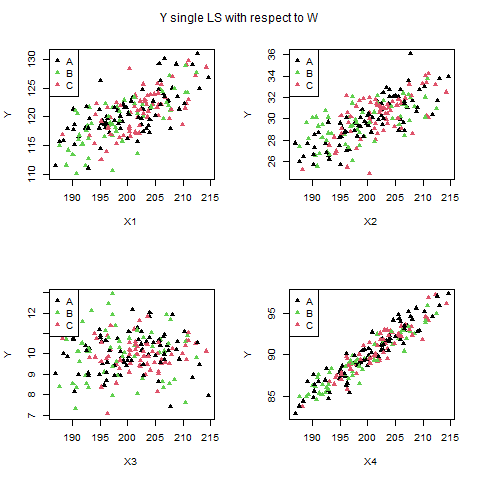
\includegraphics[width=8cm]{scatterplot_1.png}
		\centering
		\caption{Scatter-plot of Y and $X_i i=1,2,3,4$ depending on W.}
		\label{fig::scatterplot_1}
	\end{figure}
	
	
	\subsection{Simple Regression}
	
	Table \ref{tab::simple_1} shows the basic model where $Y = \beta_1 X4 + \beta_0 + \epsilon, \epsilon \sim N(0, \sigma^2)$.
	
	
% Table created by stargazer v.5.2.3 by Marek Hlavac, Social Policy Institute. E-mail: marek.hlavac at gmail.com
% Date and time: Sat, Dec 23, 2023 - 11:59:38 AM
\begin{table}[!htbp] \centering 
  \caption{Linear Regression of Y depending on X4} 
  \label{tab::simple_1} 
\begin{tabular}{@{\extracolsep{5pt}}lc} 
\\[-1.8ex]\hline 
\hline \\[-1.8ex] 
 & \multicolumn{1}{c}{\textit{Dependent variable:}} \\ 
\cline{2-2} 
\\[-1.8ex] & Y \\ 
\hline \\[-1.8ex] 
 X4 & 1.935$^{***}$ \\ 
  & p = 0.000 \\ 
  Constant & 26.197$^{***}$ \\ 
  & p = 0.00000 \\ 
 \hline \\[-1.8ex] 
Observations & 200 \\ 
R$^{2}$ & 0.886 \\ 
Adjusted R$^{2}$ & 0.886 \\ 
Residual Std. Error & 2.129 (df = 198) \\ 
F Statistic & 1,540.022$^{***}$ (df = 1; 198) \\ 
\hline 
\hline \\[-1.8ex] 
\textit{Note:}  & \multicolumn{1}{r}{$^{*}$p$<$0.1; $^{**}$p$<$0.05; $^{***}$p$<$0.01} \\ 
\end{tabular} 
\end{table} 

	
	
	\subsection{Multiple Regression}
	
	Table \ref{tab::multi_full_1} shows the full model  with base effects and interactions.
	
	
% Table created by stargazer v.5.2.3 by Marek Hlavac, Social Policy Institute. E-mail: marek.hlavac at gmail.com
% Date and time: Sat, Dec 23, 2023 - 11:59:38 AM
\begin{table}[!htbp] \centering 
  \caption{Mutiple Linear Regression of Y with main effects and interaction} 
  \label{tab::multi_full_1} 
\begin{tabular}{@{\extracolsep{5pt}}lc} 
\\[-1.8ex]\hline 
\hline \\[-1.8ex] 
 & \multicolumn{1}{c}{\textit{Dependent variable:}} \\ 
\cline{2-2} 
\\[-1.8ex] & Y \\ 
\hline \\[-1.8ex] 
 X1 & 1.168$^{***}$ \\ 
  & p = 0.00001 \\ 
  WB & $-$8.239 \\ 
  & p = 0.481 \\ 
  WC & $-$24.413$^{**}$ \\ 
  & p = 0.025 \\ 
  X2 & 2.701$^{***}$ \\ 
  & p = 0.00000 \\ 
  X3 & 0.322 \\ 
  & p = 0.166 \\ 
  X4 & $-$0.586 \\ 
  & p = 0.245 \\ 
  X1:WB & $-$0.212 \\ 
  & p = 0.538 \\ 
  X1:WC & $-$0.439 \\ 
  & p = 0.227 \\ 
  WB:X2 & $-$0.923 \\ 
  & p = 0.201 \\ 
  WC:X2 & $-$1.356$^{*}$ \\ 
  & p = 0.068 \\ 
  WB:X3 & 0.284 \\ 
  & p = 0.450 \\ 
  WC:X3 & $-$0.309 \\ 
  & p = 0.317 \\ 
  WB:X4 & 0.657 \\ 
  & p = 0.335 \\ 
  WC:X4 & 1.348$^{*}$ \\ 
  & p = 0.057 \\ 
  Constant & 28.361$^{***}$ \\ 
  & p = 0.0002 \\ 
 \hline \\[-1.8ex] 
Observations & 200 \\ 
R$^{2}$ & 0.917 \\ 
Adjusted R$^{2}$ & 0.911 \\ 
Residual Std. Error & 1.879 (df = 185) \\ 
F Statistic & 146.212$^{***}$ (df = 14; 185) \\ 
\hline 
\hline \\[-1.8ex] 
\textit{Note:}  & \multicolumn{1}{r}{$^{*}$p$<$0.1; $^{**}$p$<$0.05; $^{***}$p$<$0.01} \\ 
\end{tabular} 
\end{table} 

	
	
	\subsection{Checking the Full Model Assumptions}
	
	The model suffers from multi-collinearity ($GVIF > 10$) on most variables, meaning the model cannot be interpreted. We remove the variables with the biggest VIF scores and thus produce the model found in Table \ref{tab::multi_fixed_1}.
	
	We do not reject the normality assumption on the new model on a $95\%$ confidence level (S-W $p=0.2253$, K-S $p=0.5005$) nor the homogeneity assumption (Lev $p=0.2985$, Bart $p=0.4587$). Therefore the LS regression assumptions hold.
	
 	
% Table created by stargazer v.5.2.3 by Marek Hlavac, Social Policy Institute. E-mail: marek.hlavac at gmail.com
% Date and time: Sat, Dec 23, 2023 - 11:59:39 AM
\begin{table}[!htbp] \centering 
  \caption{Mutiple Linear Regression with no multicolinearity issues } 
  \label{tab::multi_fixed_1} 
\begin{tabular}{@{\extracolsep{5pt}}lc} 
\\[-1.8ex]\hline 
\hline \\[-1.8ex] 
 & \multicolumn{1}{c}{\textit{Dependent variable:}} \\ 
\cline{2-2} 
\\[-1.8ex] & Y \\ 
\hline \\[-1.8ex] 
 X1 & 0.968$^{***}$ \\ 
  & p = 0.000 \\ 
  X2 & 1.939$^{***}$ \\ 
  & p = 0.000 \\ 
  X3 & 0.245$^{*}$ \\ 
  & p = 0.077 \\ 
  X4 & 0.058 \\ 
  & p = 0.839 \\ 
  WB & 0.654$^{**}$ \\ 
  & p = 0.045 \\ 
  WC & 0.340 \\ 
  & p = 0.319 \\ 
  Constant & 17.944$^{***}$ \\ 
  & p = 0.0002 \\ 
 \hline \\[-1.8ex] 
Observations & 200 \\ 
R$^{2}$ & 0.909 \\ 
Adjusted R$^{2}$ & 0.907 \\ 
Residual Std. Error & 1.924 (df = 193) \\ 
F Statistic & 322.679$^{***}$ (df = 6; 193) \\ 
\hline 
\hline \\[-1.8ex] 
\textit{Note:}  & \multicolumn{1}{r}{$^{*}$p$<$0.1; $^{**}$p$<$0.05; $^{***}$p$<$0.01} \\ 
\end{tabular} 
\end{table} 

 	
 	
 	\subsection{Stepwise Model Selection}
	
	We use the stepwise selection procedure with the full model being the valid model presented in Table \ref{tab::multi_fixed_1}.
	
	The resulting model can be found in Table \ref{tab::multi_optimal_1}. Note that the dimensionality of the model has indeed been significantly reduced and that almost all terms are statistically significant on a $95\%$ confidence level.
	
	The model presents no multi-colinearity issues. We do not reject the normality assumption on the new model on a $95\%$ confidence level (S-W $p=0.2006$, K-S $p=0.6342$) nor the homogeneity assumption (Lev $p=0.4434$, Bart $p=0.4434$). Therefore the LS regression assumptions hold.
	
	
% Table created by stargazer v.5.2.3 by Marek Hlavac, Social Policy Institute. E-mail: marek.hlavac at gmail.com
% Date and time: Sat, Dec 23, 2023 - 12:04:21 PM
\begin{table}[!htbp] \centering 
  \caption{Stepwise Mutiple Linear Regression on Y} 
  \label{tab::multi_optimal_1} 
\begin{tabular}{@{\extracolsep{5pt}}lc} 
\\[-1.8ex]\hline 
\hline \\[-1.8ex] 
 & \multicolumn{1}{c}{\textit{Dependent variable:}} \\ 
\cline{2-2} 
\\[-1.8ex] & Y \\ 
\hline \\[-1.8ex] 
 X1 & 0.997$^{***}$ \\ 
  & p = 0.000 \\ 
  X2 & 1.999$^{***}$ \\ 
  & p = 0.000 \\ 
  X3 & 0.251$^{*}$ \\ 
  & p = 0.064 \\ 
  WB & 0.655$^{**}$ \\ 
  & p = 0.045 \\ 
  WC & 0.337 \\ 
  & p = 0.322 \\ 
  Constant & 17.878$^{***}$ \\ 
  & p = 0.0002 \\ 
 \hline \\[-1.8ex] 
Observations & 200 \\ 
R$^{2}$ & 0.909 \\ 
Adjusted R$^{2}$ & 0.907 \\ 
Residual Std. Error & 1.919 (df = 194) \\ 
F Statistic & 389.128$^{***}$ (df = 5; 194) \\ 
\hline 
\hline \\[-1.8ex] 
\textit{Note:}  & \multicolumn{1}{r}{$^{*}$p$<$0.1; $^{**}$p$<$0.05; $^{***}$p$<$0.01} \\ 
\end{tabular} 
\end{table} 

	
	
	\subsection{Estimating Y}
	
	When $X1=120, X2=30, X3=10, X4=90, W=B$ the stepwise model presented in Table \ref{tab::multi_optimal_1} predicts a value of $Y=200.6143$ with a $95\%$ confidence interval of $(200.1456 \leq Y \leq 201.083)$.
	
	
	\subsection{Categorizing Continuous Variable}
	The contingency table can be found in \ref{fig::contigency_1}.
	
	Executing the two-way ANOVA test between Y and W*Z, we determine that there are statistically significant differences in the means of Y depending on the two variables on a $95\%$ confidence interval (W: $p=5.12e-09$, Z: $p=0$) but not their interaction (W:Z $p= 0.305$). Therefore while the means deviate, the slope of Y to Z and Y to W does not change.
	
	We do not reject the normality assumption on the ANOVA test on a $95\%$ confidence level (S-W $p=0.8318$, K-S $p=0.9147$) nor the homogeneity assumption (Lev $p=0.6634$). Therefore the ANOVA assumptions hold.
	
	\begin{figure}
		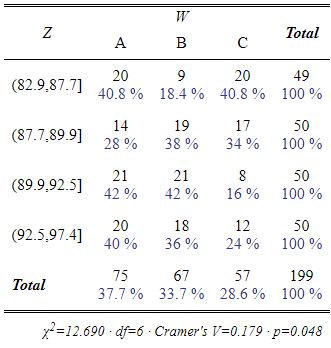
\includegraphics[width=8cm]{contigency_1.png}
		\centering
		\caption{Contingency table between W and Z (quantiles of X4)}
		\label{fig::contigency_1}
	\end{figure}
	
\end{document}